\documentclass[border=10pt]{standalone}
\usepackage{fontspec}\usepackage{tikz}
\usetikzlibrary{arrows.meta,positioning,calc}
\definecolor{NouOrange}{HTML}{FA4D1F}\definecolor{NouBlack}{HTML}{000000}
\begin{document}
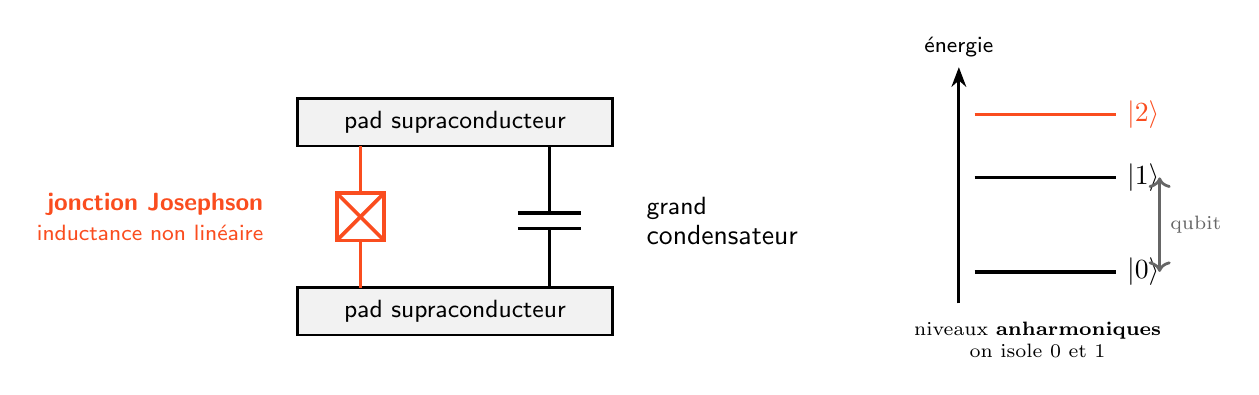
\begin{tikzpicture}[font=\sffamily,line width=1pt]
  % --- Circuit : deux pads relies par une JJ (gauche) et un condensateur (droite) ---
  \draw[NouBlack,fill=black!5] (0,2.2) rectangle (4,2.8);   % pad haut
  \draw[NouBlack,fill=black!5] (0,-0.2) rectangle (4,0.4);  % pad bas
  \node at (2,2.5){\small pad supraconducteur};
  \node at (2,0.1){\small pad supraconducteur};
  % jonction Josephson (croix dans un carre) a gauche
  \draw[NouOrange,line width=1.3pt] (0.8,0.4) -- (0.8,1.0);
  \draw[NouOrange,line width=1.3pt] (0.8,1.6) -- (0.8,2.2);
  \draw[NouOrange,line width=1.3pt] (0.5,1.0) rectangle (1.1,1.6);
  \draw[NouOrange,line width=1.3pt] (0.5,1.0) -- (1.1,1.6);
  \draw[NouOrange,line width=1.3pt] (0.5,1.6) -- (1.1,1.0);
  \node[NouOrange,anchor=east,align=right] at (-0.3,1.3){\small\textbf{jonction Josephson}\\[-1pt]{\footnotesize inductance non linéaire}};
  % condensateur a droite
  \draw[NouBlack,line width=1.3pt] (3.2,0.4) -- (3.2,1.15);
  \draw[NouBlack,line width=1.3pt] (2.8,1.15) -- (3.6,1.15);
  \draw[NouBlack,line width=1.3pt] (2.8,1.35) -- (3.6,1.35);
  \draw[NouBlack,line width=1.3pt] (3.2,1.35) -- (3.2,2.2);
  \node[anchor=west,align=left] at (4.3,1.25){\small grand\\[-1pt]condensateur};
  % --- Echelle d'energie anharmonique a droite ---
  \begin{scope}[xshift=8.4cm,yshift=0.2cm]
    \draw[-{Stealth[length=2.5mm]},NouBlack] (0,0) -- (0,3) node[above]{\footnotesize énergie};
    \draw[NouBlack,line width=1.2pt] (0.2,0.4) -- (2,0.4) node[right]{$|0\rangle$};
    \draw[NouBlack,line width=1.2pt] (0.2,1.6) -- (2,1.6) node[right]{$|1\rangle$};
    \draw[NouOrange,line width=1.2pt] (0.2,2.4) -- (2,2.4) node[right]{$|2\rangle$};
    \draw[<->,NouBlack!60] (2.55,0.4) -- (2.55,1.6) node[midway,right,font=\scriptsize]{qubit};
    \node[below=3pt of {(1,0)},anchor=north,align=center,font=\scriptsize]{niveaux \textbf{anharmoniques}\\on isole 0 et 1};
  \end{scope}
\end{tikzpicture}
\end{document}
